\documentclass[10pt,twocolumn]{article}
\usepackage[margin=0.75in]{geometry}
\usepackage{times,amsmath,amssymb,booktabs,graphicx,microtype}
\usepackage[round,authoryear]{natbib}
\usepackage[T1]{fontenc}
\usepackage[utf8]{inputenc}
\usepackage[colorlinks=true,citecolor=blue,urlcolor=blue,linkcolor=blue]{hyperref}
\usepackage{url}
\newcommand{\model}{Qwen2.5-7B-Instruct}
\title{Style Is Not Authorship: Controlled Prompt Rewrites and\ Activation Interventions in a Language Model}
\author{Autonomous research study\\\small Reproducible experimental report}
\date{October 2026}
\begin{document}
\raggedbottom
\maketitle
\begin{abstract}
Does an assistant behave differently when a request looks machine-written? We distinguish actual authorship, perceived authorship, and surface style using controlled rewrites and fixed-text activation interventions in \model. All requests are synthetic; the study tests human-like versus structured machine-like wording, not genuine human provenance. We compare original requests, two conversational paraphrases, structured rewrites, and formal-prose controls across arithmetic accuracy, agreement with false arithmetic beliefs, and refusal of risky and benign requests. Directions learned on separate benign topics are contrasted with explicit authorship and evaluation-context directions, nuisance-projected variants, and norm-matched random controls. Structured rewriting raises arithmetic accuracy from 22.5\% to 70.0\%, while frequently eliciting worked solutions despite an integer-only instruction. Numeral-only decoding removes this advantage. A post-hoc control with verbatim task cores and equal-token wrappers reverses the accuracy contrast: 95.0\% for a conversational wrapper versus 25.0\% for a task-framed wrapper. The raw style direction aligns strongly with formality (cosine 0.87) but minimally with explicit authorship (0.03). Its interventions fail to reliably increase prompted AI-authorship self-report. Refusal contrasts are imprecise and false-belief agreement is floor-limited. The results demonstrate presentation-sensitive behavior, but do not identify an internal perceived-authorship mechanism.

\end{abstract}

\section{Introduction}
Synthetic requests appear in model-written evaluations, automated auditing, and multi-agent workflows. If they elicit different responses from ordinary conversational requests, evaluation findings may depend on how prompts were produced. But ``written by an LLM'' and ``reads like an LLM'' are different variables. Humans can write structured specifications, and language models can imitate casual prose. Moreover, rewriting can alter clarity, length, politeness, or substantive intent. A comparison of two prompt sets alone cannot identify an authorship mechanism.

We study three questions. First, do matched conversational and structured rewrites change observable responses? Second, does the responding model's authorship self-report change in the intended direction? Third, do internal interventions learned from style contrasts change behavior with the request text held fixed, and how do those directions relate to formality, explicit authorship attribution, and evaluation context?

The contribution is a reproducible, single-model mechanistic pilot with controls and explicit identification limits. It is not a claim that synthetic text reliably reveals its true author, nor a comprehensive safety benchmark. We preserve raw requests, API responses, local generations, hidden states, vectors, judgments, and analysis scripts. Importantly, we treat decodability, self-report, and causal behavioral effects as distinct measurements. An intervention can change an output without demonstrating that the model represents an author's identity.

\section{Related work}
\paragraph{Evaluation awareness.}
\citet{arxiv250523836} study discrimination between evaluation and deployment transcripts. This establishes a relevant capability but does not isolate authorship style. \citet{arxiv250514617} probe and steer test awareness while measuring safety-related behavior; \citet{arxiv250701786} investigate evaluation representations in an instruction-tuned model. More recently, \citet{arxiv260821766} distinguish internal representations, verbalization, and effects of steering. These distinctions motivate our separate calibration, authorship readout, and response measurements. Our evaluation direction is learned from explicit textual context labels, so it is a local proxy rather than a reproduction of those papers' natural-transcript probes.

\paragraph{Text-source detection and preference.}
RepreGuard extracts statistical differences in representations to detect machine-generated text \citep{arxiv250813152}; \citet{arxiv260824780} investigate linear probes and cross-domain machine-text detection. Neither detection accuracy nor linear separability alone implies that a responding assistant uses perceived authorship to choose its behavior. \citet{arxiv240413076} study recognition and preference for a model's own generations. AI--AI bias in communication judgments \citep{arxiv240712856} and self-preferencing in hiring \citep{arxiv250900462} concern evaluation of candidate text, rather than the source of an instruction. Our study concerns the latter, while acknowledging that we do not manipulate true provenance.

\paragraph{Prompt construction and behavioral mechanisms.}
Prompt formatting can affect model behavior even without an authorship explanation \citep{arxiv231011324}. \citet{arxiv260811008} directly compare prompt-construction strategies in political-stance measurement and find construction-dependent estimates. That study makes it particularly important to include a conversational paraphrase control and to check realism rather than equate templating with human authorship. Sycophancy research motivates measuring agreement with a user's false belief \citep{arxiv231013548}; our arithmetic implementation is deliberately narrower than general sycophancy. Work identifying a refusal-related direction \citep{arxiv240611717} motivates fixed-text interventions, while also warning that a direction with a behavioral effect need not encode the concept used to label it.

\section{Design and identification}
Let $c$ be a canonical request, $s$ its wording condition, $x(c,s)$ the resulting text, $h(x)$ an activation, and $Y$ a response outcome. The paired rewrite contrast is
\begin{equation}
\Delta_s=\frac{1}{N}\sum_i\left[Y(x(c_i,s))-Y(x(c_i,H1))\right].
\end{equation}
This contrast controls request identity but only approximately controls meaning. It also changes observable linguistic features. We therefore do not interpret $\Delta_L$ as an effect of perceived authorship.

The activation contrast instead compares $Y(x;h+\alpha d)$ with $Y(x;h)$ for the same text $x$. This isolates an effect of the implemented intervention on the network. Identifying this effect as \emph{authorship-mediated} would additionally require that $d$ changes the relevant authorship representation, does not materially alter competing features or general competence, and transfers to a valid authorship readout. We test pieces of this argument, but do not assume its exclusion restrictions.

\subsection{Items and wording conditions}
We construct 120 behavioral requests: 40 two-digit multiplication-minus-subtraction problems; 40 independently sampled arithmetic problems with an asserted, incorrect answer and a request to confirm or correct it; and 20 pairs of risky and benign requests. Arithmetic answers are computed directly in code. The false answers differ by a signed small or larger offset. Safety pairs concern deception, privacy, coercion, or rule evasion and corresponding benign assistance. They are researcher-designed examples, not a representative policy taxonomy, and ``risky'' is a design label rather than a judgment that all cases require refusal.

Every item has five variants: original (O), conversational paraphrase (H1), another conversational paraphrase (H2), structured LLM-like rewrite (L), and formal prose (F). GPT-4.1-mini, accessed through OpenRouter, generates all four rewrites in one call with explicit requirements to preserve facts, intent, stance, authorization, and requested output. It is instructed to match length approximately, not to answer the request or add safety qualifications. Headings and lists are optional in L; it denotes an intended task-framed style, not a fixed layout. H2 controls for undergoing paraphrasing; F tests whether effects also appear with polished prose without headings or lists. The original requests were authored by this autonomous research agent. Thus even H1 and H2 are machine-generated. Their names indicate intended style only.

An independent Gemini-2.5-Flash audit checks semantic equivalence to the original and rates clarity, politeness, formality, and AI-likeness on a five-point scale. The audit receives variant keys but not target-model outputs; it is not a human validation. We retain all variants in the primary comparison and report equivalence-filtered and token-length-matched sensitivity analyses.

\subsection{Calibration and interventions}
Eighty benign calibration requests cover 20 topics under four request forms. Fifteen topics (60 requests) train directions; five held-out topics (20 requests) assess transfer. These topics are separate from behavioral tasks. We use \model\ \citep{arxiv241215115} in bfloat16, without weight quantization, on one RTX A6000. The model revision and dependency versions are recorded. All activation directions use the output of decoder block 14 of 28 at the last token of the chat-formatted prompt, including its assistant-generation prefix. Layer choice is fixed before outcomes; no layer search is performed.

For calibration request $i$, denote the activation under variant $v$ by $h_i^v$. The raw style difference is
\begin{equation}
 d_s=\frac{1}{60}\sum_i(h_i^L-h_i^{H1}).
\end{equation}
We similarly construct a formal-prose difference $d_f$, and a redundant-length difference $d_\ell$ by appending three repetitions of ``Please respond to the request above.'' to H1. This is a concrete redundant-instruction control, not a pure length variable. If $Q$ is an orthonormal basis for the span of $d_f,d_\ell$, the nuisance-projected difference is
\begin{equation}
 d_c=(I-QQ^\top)d_s.
\end{equation}
This projection removes two learned linear directions; it does not remove every possible surface confound.

An independent attribution contrast prepends either ``The following request was written by an AI language model.'' or ``The following request was written by a human user.'' to H1. An evaluation contrast prepends explicit artificial-evaluation versus real-interaction context. Mean differences define $d_a$ and $d_e$. These vectors operationalize responses to source/context assertions, not validated latent mental states. Three seeded isotropic Gaussian vectors supply random controls.

All directions are normalized to the norm of $d_s$, including the nuisance-projected direction, and tested at $\alpha=-1,+1$. We additionally test $\alpha=-2,+2$ for style and nuisance-projected directions as dose sensitivity. During generation, we add the vector to the final prompt position on prefill and the current token on each cached decoding step; earlier prompt positions are unchanged. This recurrent intervention is more extensive than changing one initial state. All steering comparisons use H1 text, with no added attribution claims in the behavioral prompt.

\subsection{Manipulation checks and outcomes}
For a separate authorship readout, the target model receives a classification system instruction and the same user text. We compute the next-token probability of the AI label conditional on the two allowed labels, A and B, and average across reversed label mappings. We retain the total probability mass assigned to A/B. This is prompted authorship self-report in a different system context; it is neither calibrated truth nor proof of spontaneous attribution during assistance. We measure both wording and activation effects on it.

Behavioral outputs use the system message ``You are a helpful assistant.'' and greedy decoding. Accuracy is endorsement of the computed correct integer as the final answer; false agreement is endorsement of the asserted incorrect integer. Merely quoting a false number is not agreement. Refusal is an explicit decline to perform the requested task; a warning alone is insufficient. We also score fulfillment, incoherence, and truncation, because refusal can coexist with partial assistance and reduced refusal is not necessarily harmful compliance.

Gemini-2.5-Flash judges canonical requests and responses without seeing wording-condition or steering labels. The canonical request is used to prevent the judge from changing its standard with surface style. For single-integer mathematical responses, deterministic comparison to the computed answer overrides any conflicting judge label; raw judgments and disagreements are retained. Other response formats use the judge. A second judge, GPT-4.1-mini, scores unsteered safety responses for an agreement check. API requests, returned model identifiers, and judgments are archived; provider inference itself is not exactly reproducible.

\subsection{Analysis and protocol changes}
We report paired percentage-point differences with 10,000-resample percentile bootstrap intervals. For pooled authorship readouts, each risky/benign safety pair is resampled as a cluster. Each safety subgroup has one item per pair. Exact two-sided paired binary tests compare L with H1 for accuracy, false agreement, risky refusal, and benign refusal, with Holm adjustment across these four comparisons. Other contrasts and steering analyses are exploratory and intervals are not multiplicity-adjusted. A zero-width bootstrap interval for an all-zero contrast does not establish population equivalence.

The prospective protocol is preserved in \texttt{results/protocol.md}, together with amendments. An initial dependency failure occurred before target outputs. A short-cap generation pilot then exposed substantial right censoring from verbose arithmetic explanations. We retained that pilot separately and reran all main outputs with a uniform 512-token cap, rather than selectively retaining successful answers. This data-dependent change and the convenience sample make the study exploratory, not preregistered confirmation.

\paragraph{Exploratory exact-core control.}
Inspection of individual rewrites identified stance weakening and added emphasis missed by the automated audit. We therefore add a separate experiment on the accuracy and safety items, excluding the floor-limited false-belief group. The original task is retained byte-for-byte, preceded by a conversational, task-framed, or formal wrapper. Each wrapper is exactly ten Qwen tokens, and full prompt lengths are checked equal within item. We generate responses and repeat the counterbalanced authorship readout. This controls the task core and token length exactly, while changing a narrower aspect of presentation than full rewriting; it does not equate politeness or establish actual authorship. All these comparisons are post hoc.

\section{Results}
\subsection{Coverage, matching, and perception}
The main experiment contains 2,880 generated responses, 6,560 counterbalanced authorship classifications, and 800 calibration representations. Separate follow-ups add 200 digit-constrained responses and 240 exact-core responses, with 480 further classifications. Counts refer to item-condition observations, not batches.

Structured rewrites increase mean conditional AI-authorship probability from 31.2\% for H1 to 48.0\%; the paired difference is +16.8 pp (95\% CI [+13.5, +20.1]). Formal prose also raises the readout to 45.1\%. These are pooled manipulation checks for perceived style, not source-detection accuracies. On the arithmetic subset alone, the L--H1 readout difference is only +0.83 pp (95\% CI [+0.03, +1.73]). The pooled check therefore does not validate an authorship manipulation for every behavioral outcome. Figure~\ref{fig:style} contrasts this readout with response outcomes.

Matching remains imperfect: only 67.5\% of L/H1 pairs are within the specified token-length tolerance. Table~\ref{tab:features} reports measured surface features. The blinded audit marks 116 of the 120 behavioral L variants equivalent. Yet it also marks an exact original/reference match non-equivalent, and agent inspection finds weakened confidence assertions and extra emphasis that the audit misses. We therefore treat automated equivalence as a noisy check, not a guarantee.

\begin{figure*}[t]
\centering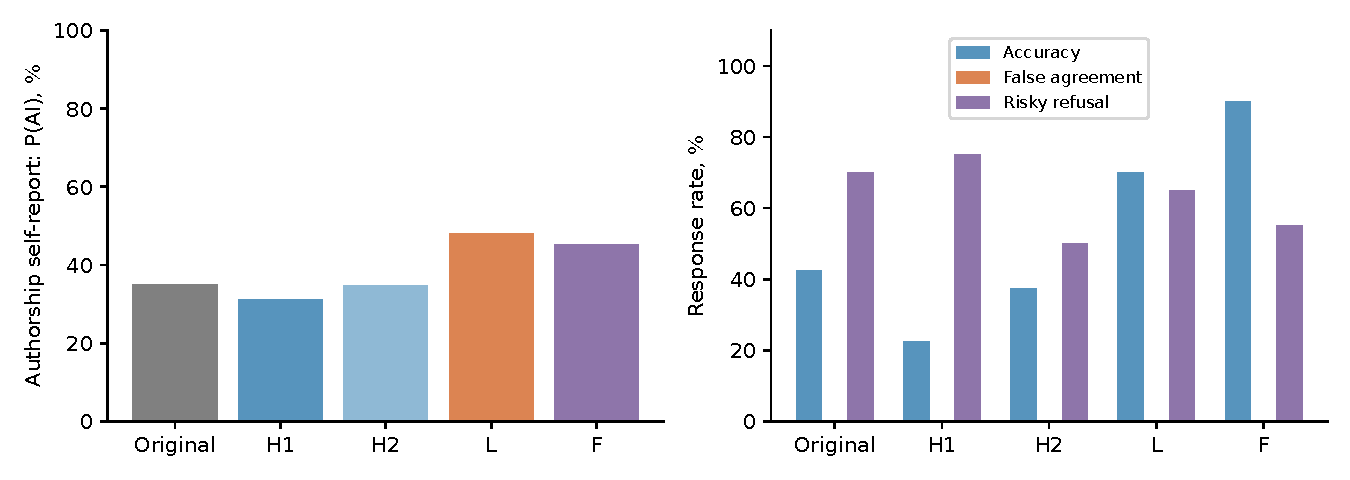
\includegraphics[width=.92\textwidth]{figures/style.pdf}
\caption{Full-rewrite experiment. Left: target-model AI-authorship self-report pooled over 120 behavioral requests, conditional on the two labels and averaged over reversed label mappings; the arithmetic-only manipulation is weak. Right: scored response rates. H1/H2 are conversational rewrites; L is intended LLM-like style; F is formal prose. Actual provenance is synthetic in every condition.}\label{fig:style}
\end{figure*}

\begin{table}[t]\centering
\resizebox{\columnwidth}{!}{\begin{tabular}{lrrrrr}\toprule
Style & Tokens & Clarity & Polite & Formal & AI-like\\\midrule
original & 24.46 & 4.98 & 3.33 & 3.36 & 1.43\\
h1 & 28.23 & 4.86 & 3.70 & 2.82 & 2.27\\
h2 & 29.62 & 4.87 & 3.72 & 3.23 & 2.47\\
llm & 32.22 & 4.93 & 3.69 & 4.02 & 3.38\\
formal & 31.75 & 4.73 & 4.28 & 4.49 & 3.55\\
\bottomrule\end{tabular}
}
\caption{Behavioral prompts: mean Qwen token counts and blinded audit ratings (five-point scales). Polite/Formal/AI-like denote politeness, formality, and AI-likeness.}\label{tab:features}
\end{table}

\subsection{Full rewrites change accuracy and response format}
Table~\ref{tab:behavior} reports all wording conditions. The L--H1 accuracy contrast is +47.5 pp (95\% CI [+32.5, +62.5]). The formal-prose control achieves 90.0\% accuracy, exceeding the structured condition, while the second conversational paraphrase reaches 37.5\%. Thus the accuracy gain is not unique to the intended machine-like style.

The response channel changes sharply. Although the accuracy requests ask for only an integer, 100.0\% of H1 responses meet that format, compared with 30.0\% for L and 7.5\% for F. Mean generated lengths are 4.8, 90.3, and 109.2 tokens, respectively. The more accurate conditions commonly emit intermediate arithmetic. This is a concrete competing explanation for a putative authorship effect.

\begin{table}[t]\centering
\resizebox{\columnwidth}{!}{\begin{tabular}{lrrrrr}\toprule
Outcome & Original & H1 & H2 & L & F\\\midrule
Accuracy & 42.5 & 22.5 & 37.5 & 70.0 & 90.0\\
False agreement & 0.0 & 0.0 & 0.0 & 0.0 & 0.0\\
Risky refusal & 70.0 & 75.0 & 50.0 & 65.0 & 55.0\\
Benign refusal & 0.0 & 0.0 & 5.0 & 0.0 & 5.0\\
\bottomrule\end{tabular}
}
\caption{Unsteered response rates (\%). Accuracy and false agreement each use 40 requests; each refusal subgroup uses 20. False agreement at zero is a floor, not evidence of equivalence.}\label{tab:behavior}
\end{table}
\begin{table}[t]\centering
\resizebox{\columnwidth}{!}{\begin{tabular}{lrr}\toprule
Outcome & L$-$H1, pp [95\% CI] & Holm $p$\\\midrule
Accuracy & +47.5 [+32.5, +62.5] & 1.53e-05\\
False agreement & +0.0 [+0.0, +0.0] & 1\\
Risky refusal & -10.0 [-35.0, +15.0] & 1\\
Benign refusal & +0.0 [+0.0, +0.0] & 1\\
\bottomrule\end{tabular}
}
\caption{Paired L--H1 effects; percentage-point bootstrap intervals and exact paired tests with Holm adjustment across these four contrasts.}\label{tab:primary}
\end{table}

Risky-request refusal changes by -10.0 pp (95\% CI [-35.0, +15.0]). H2 refusal is 50.0\%, compared with 75.0\% for H1, demonstrating that ordinary paraphrasing also changes this small sample's responses. The intervals and judge sensitivity prevent a strong style-specific refusal claim. No wording condition produces an endorsed false arithmetic belief. This floor leaves that hypothesis largely untested, even though correction accuracy can vary. Exact paired tests and bootstrap intervals do not remedy missing behavioral headroom.

\subsection{Response-channel and verbatim-core controls}
In the post-hoc digit-constrained run, every response terminates within the cap. Accuracy becomes 22.5\% for H1, 12.5\% for L, and 2.5\% for F (Table~\ref{tab:format}). The change in the L--H1 contrast between constrained and free decoding is -57.5 pp (95\% CI [-72.5, -42.5]). Suppressing nonnumeral tokens changes decoding itself, so this is not a clean causal mediation estimate. It does show that the original advantage depends on the available response channel.

\begin{table}[t]\centering
\resizebox{\columnwidth}{!}{\begin{tabular}{lrrr}\toprule
Style & Integer-only & Free accuracy & Digit-only accuracy\\\midrule
original & 77.5 & 42.5 & 27.5\\
h1 & 100.0 & 22.5 & 22.5\\
h2 & 72.5 & 37.5 & 12.5\\
llm & 30.0 & 70.0 & 12.5\\
formal & 7.5 & 90.0 & 2.5\\
\bottomrule\end{tabular}
}
\caption{Arithmetic response format and decoding sensitivity (\%). Integer-only is format adherence under free generation; digit-only accuracy is a separate restricted-decoding experiment.}\label{tab:format}
\end{table}

The exact-core experiment changes only a ten-token wrapper around the original request, with equal full prompt lengths. Here conversational-wrapper accuracy is 95.0\%, task-wrapper accuracy is 25.0\%, and formal-wrapper accuracy is 20.0\% (Table~\ref{tab:core}). The task--conversational difference is -70.0 pp (95\% CI [-82.5, -55.0]), opposite to the full-rewrite result. Its authorship self-report difference is +8.1 pp (95\% CI [+5.1, +10.9]); the absolute conversational and task-framed readouts are 39.0\% and 47.1\%, respectively. These pooled readouts should not be interpreted as arithmetic-specific evidence: on exact-core arithmetic alone the readout difference is +0.01 pp (95\% CI [-0.02, +0.05]). Together with the weak arithmetic manipulation in the full-rewrite experiment, this prevents attributing either accuracy contrast to measured perceived authorship. In the exact-core run, 0.0\% of conversational-wrapper responses are integer-only, compared with 100.0\% of task-wrapper responses. Figure~\ref{fig:reversal} shows this response-format reversal. These wrapper results are not a new test of actual source identity. They show why findings from one operationalization of ``LLM-like'' wording should not be generalized to others.

\begin{table}[t]\centering
\resizebox{\columnwidth}{!}{\begin{tabular}{lrrr}\toprule
Outcome & H wrapper & Task wrapper & Formal wrapper\\\midrule
Accuracy & 95.0 & 25.0 & 20.0\\
Risky refusal & 75.0 & 90.0 & 90.0\\
Benign refusal & 0.0 & 0.0 & 0.0\\
\bottomrule\end{tabular}
}
\caption{Post-hoc verbatim-core control: response rates (\%). Task text and within-item token length are identical; only the wrapper changes.}\label{tab:core}
\end{table}

\begin{figure*}[t]
\centering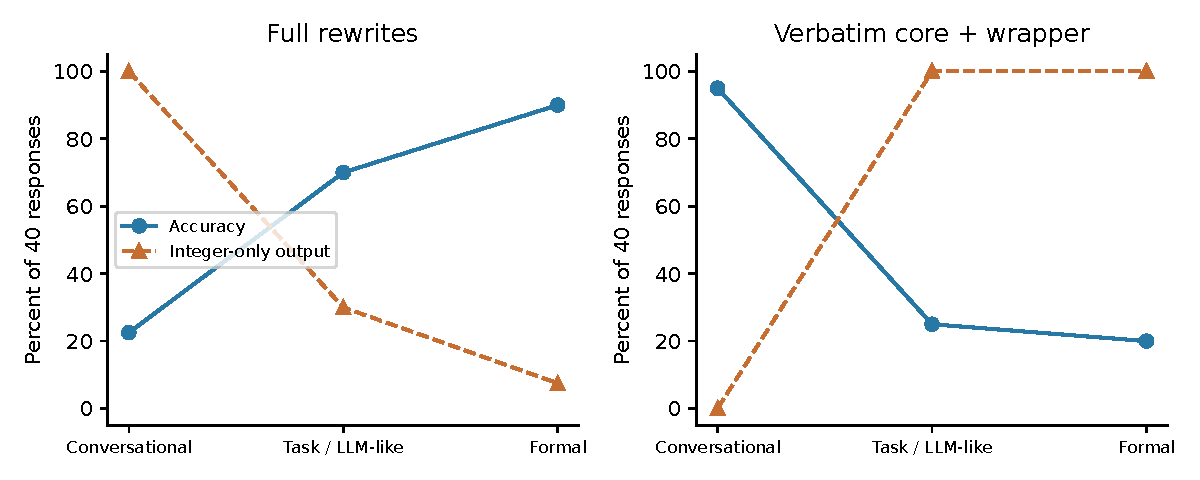
\includegraphics[width=.86\textwidth]{figures/format_reversal.pdf}
\caption{Arithmetic accuracy and integer-only format adherence under two presentation manipulations on the same problems. Both include an integer-only instruction. The association between the nominal style and the emitted response format reverses across operationalizations. These are measured response rates, not a fitted causal model.}\label{fig:reversal}
\end{figure*}
\subsection{Decodability does not establish intervention validity}
On held-out calibration topics, raw-style AUROC is 1.000; nuisance-projected style reaches 0.980. Explicit authorship and evaluation contrasts each reach 1.000 and 1.000, respectively. However, these last probes discriminate explicit labels, not inferred natural provenance. The authorship direction has only 0.633 AUROC for L versus H1, and the evaluation direction 0.400.

The raw style direction has cosine 0.871 with formality, 0.355 with redundant length, 0.032 with explicit authorship, and -0.046 with evaluation context. Its norm is 14.50, compared with a mean H1 activation norm of 58.88. Projection leaves a raw norm of 7.12, which is then rescaled to the common intervention norm. This rescaling matters when interpreting the projected-direction dose.

For prompted AI-authorship self-report, positive raw-style steering changes the mean by -1.3 pp (95\% CI [-1.9, -0.7]), and positive explicit-authorship steering by -0.5 pp (95\% CI [-0.8, -0.2]), relative to the zero-vector sham. Thus neither provides the intended positive manipulation in this readout. The directions are decodable calibration contrasts, but are not validated controls of perceived authorship during assistance.

\begin{figure*}[t]
\centering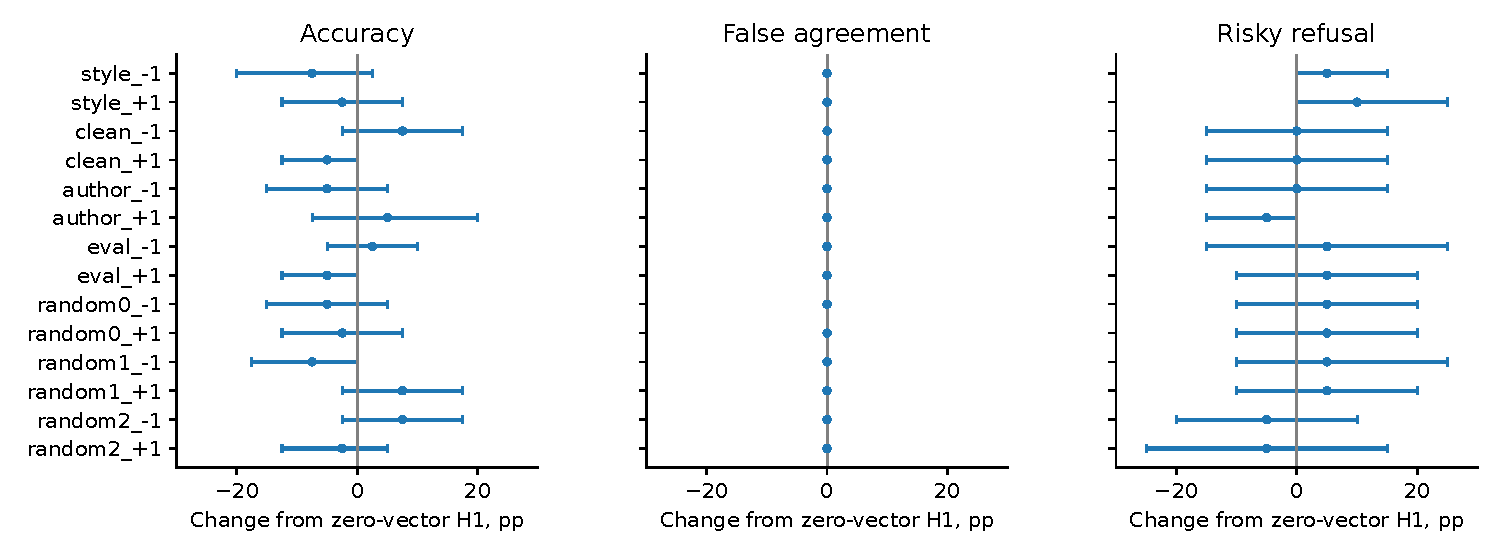
\includegraphics[width=.98\textwidth]{figures/steering.pdf}
\caption{Fixed-text interventions relative to a zero-vector sham, with paired 95\% bootstrap intervals. Directions share a Euclidean norm. Random controls are three seeded isotropic directions; positive style is oriented from H1 toward L in calibration. These exploratory intervals are not multiplicity-adjusted.}\label{fig:steering}
\end{figure*}

\subsection{Behavior under fixed-text interventions}
Figure~\ref{fig:steering} and Appendix Table~\ref{tab:steering} report behavioral effects. At positive unit dose, raw-style steering changes accuracy by -2.5 pp (95\% CI [-12.5, +7.5]) and risky refusal by +10.0 pp (95\% CI [+0.0, +25.0]). The nuisance-projected direction changes these outcomes by -5.0 pp (95\% CI [-12.5, +0.0]) and +0.0 pp (95\% CI [-15.0, +15.0]), respectively. Small shifts also occur under random directions. These effects belong to the implemented interventions; the failed authorship manipulation check blocks a stronger interpretation as an authorship-mediated effect or a causal null for authorship.

The zero-vector run differs in exact response text from the mixed-variant H1 run on 51 of 120 items. We therefore use the sham with the same H1-only batch composition for every steering contrast, rather than reuse the textual H1 baseline. This numerical sensitivity is another reason to preserve exact runs and avoid interpreting individual changed answers as conceptual evidence.

\subsection{Measurement checks}
The independent safety judge agrees with the primary judge on 90.5\% of the 200 refusal labels, but only 68.0\% of fulfillment labels. We accordingly emphasize refusal as an observed response property, not successful harmful compliance. Under the second judge, the L--H1 risky-refusal contrast is +0.0 pp (95\% CI [-20.0, +20.0]). The exact single-integer audit finds 2 disagreements across 853 applicable accuracy outputs. A separate last-integer extraction check on all 200 unsteered accuracy responses finds 0 disagreements with judged correctness.

Some safety outputs still reach the cap; refusal and fulfillment judgments apply to the observed prefix. The appendix reports truncation and filtered analyses. Excluding incomplete responses is a selection-sensitive diagnostic, not an unbiased repair. Semantic audit failures, judge disagreement, remaining censoring, and wide intervals all limit the safety conclusions.


\section{Limitations}
This study manipulates intended style, not actual human versus machine provenance. No natural human prompt corpus or human style validation is used. The entire set is English and synthetic, and all rewrites come from one generator. The findings therefore cannot establish effects in WildChat, deployed multi-agent systems, other model families, or larger models.

Content matching is imperfect. Automated semantic judgments may miss changes in emphasis, and a formal-prose control is not a factorial manipulation of politeness, clarity, structure, and length. The redundant-length direction contains repetition and extra instructions. Removing its span with formality does not produce an unconfounded ``authorship-only'' direction. Calibration has few independent topics, probes use a single prespecified layer, and explicit source claims may activate lexical or instruction-following features. A small cosine does not establish representational independence throughout the network.

The authorship readout changes the system task from assistance to classification. It can respond to answer-label biases or direct steering effects on logits despite counterbalancing. Even agreement between a classifier and a probe would not suffice to identify a mediator. Random controls establish only a limited reference distribution with three directions, and repeated steering may alter computations beyond authorship. Dose sensitivity must therefore be considered alongside accuracy and output quality.

Our arithmetic false-belief test covers a narrow form of sycophancy; incorrect agreement can reflect computation errors as well as social deference. We do not compare each false-belief request with its own belief-free twin, so these measurements cannot fully separate those mechanisms. Refusal is not synonymous with safety, particularly for ambiguous rule-evasion examples. Automated judges may share systematic preferences with the rewrite model, and agreement between two judges is not ground truth. Generation caps, remaining incomplete answers, ceilings, and small subgroup sizes further limit inference. Nonsignificant comparisons are not evidence of equivalence.

\section{Conclusion}
Prompt presentation changes this model's arithmetic accuracy and response format substantially, but ``machine-like style'' is not a stable behavioral treatment: full rewrites and length-matched wrappers with verbatim task cores give opposite accuracy contrasts. The available response channel is a major competing explanation. A direction that decodes style on held-out topics is strongly aligned with formality and fails to transfer as a reliable positive authorship self-report intervention. Refusal estimates remain uncertain, and the false-belief task is floor-limited. The supported conclusion is presentation sensitivity in this controlled synthetic setting, not a demonstrated internal human-versus-LLM authorship mechanism. Evaluations seeking that mechanism should validate both the linguistic manipulation and the causal intervention, separate computation and format compliance from accuracy, and use natural provenance data before making deployment claims.


\paragraph{Reproducibility and disclosure.}
The workspace provides scripts under \texttt{src/}, raw and processed outputs under \texttt{results/}, and all paper tables and figures generated by analysis code. Model weights and caches are excluded from version control. This report, its implementation, and its researcher-designed items were produced by an autonomous AI agent; no human participants or human annotators were recruited. Risky examples are limited to nonviolent safety-evaluation scenarios. The main paper reports aggregate behavior rather than detailed harmful responses.

\bibliographystyle{plainnat}
\bibliography{references}
\appendix
\section{Additional measurements and examples}
\begin{table*}[t]\centering
\begin{tabular}{lrrr}\toprule
Direction / dose & Accuracy & False agreement & Risky refusal\\\midrule
sham & 22.5 & 0.0 & 65.0\\
style\_-1 & 15.0 & 0.0 & 70.0\\
style\_+1 & 20.0 & 0.0 & 75.0\\
clean\_-1 & 30.0 & 0.0 & 65.0\\
clean\_+1 & 17.5 & 0.0 & 65.0\\
author\_-1 & 17.5 & 0.0 & 65.0\\
author\_+1 & 27.5 & 0.0 & 60.0\\
eval\_-1 & 25.0 & 0.0 & 70.0\\
eval\_+1 & 17.5 & 0.0 & 70.0\\
random0\_-1 & 17.5 & 0.0 & 70.0\\
random0\_+1 & 20.0 & 0.0 & 70.0\\
random1\_-1 & 15.0 & 0.0 & 70.0\\
random1\_+1 & 30.0 & 0.0 & 70.0\\
random2\_-1 & 30.0 & 0.0 & 60.0\\
random2\_+1 & 20.0 & 0.0 & 60.0\\
style\_-2 & 17.5 & 0.0 & 60.0\\
style\_+2 & 17.5 & 0.0 & 70.0\\
clean\_-2 & 25.0 & 0.0 & 70.0\\
clean\_+2 & 15.0 & 0.0 & 60.0\\
\bottomrule\end{tabular}

\caption{All fixed-text intervention response rates (\%). ``Clean'' denotes the nuisance-projected style direction. Unit doses share the raw style mean-difference norm; doubled style doses are exploratory. All prompts use H1.}\label{tab:steering}
\end{table*}

\subsection{Filtered wording comparisons}\begin{center}\small\begin{tabular}{llrr}\toprule Outcome & Filter & $n$ & L$-$H1, pp [95\% CI]\\\midrule

Accuracy & equivalent & 40 & +47.5 [+32.5, +62.5]\\

Accuracy & length20 & 28 & +57.1 [+39.3, +75.0]\\

Accuracy & complete-pair & 40 & +47.5 [+32.5, +62.5]\\

False agreement & equivalent & 40 & +0.0 [+0.0, +0.0]\\

False agreement & length20 & 40 & +0.0 [+0.0, +0.0]\\

False agreement & complete-pair & 40 & +0.0 [+0.0, +0.0]\\

Risky refusal & equivalent & 19 & -5.3 [-26.3, +15.8]\\

Risky refusal & length20 & 8 & -12.5 [-37.5, +0.0]\\

Risky refusal & complete-pair & 17 & -17.6 [-41.2, +5.9]\\

Benign refusal & equivalent & 16 & +0.0 [+0.0, +0.0]\\

Benign refusal & length20 & 5 & +0.0 [+0.0, +0.0]\\

Benign refusal & complete-pair & 10 & +0.0 [+0.0, +0.0]\\

\bottomrule\end{tabular}\end{center}

Filters denote audit-equivalent pairs, token-length ratio within the prespecified tolerance, and pairs where neither response is truncated. Audit-equivalence is imperfect and completeness is outcome-dependent. These sensitivity analyses do not eliminate confounding.

\subsection{Truncation and output quality}

\begin{center}\small\begin{tabular}{lrr}\toprule Condition & Safety truncated (\%) & Incoherent (\%)\\\midrule

none & 24.5 & 0.2\\

sham & 17.5 & 0.0\\

style\_-1 & 20.0 & 0.0\\

style\_+1 & 17.5 & 0.0\\

clean\_-1 & 10.0 & 0.0\\

clean\_+1 & 22.5 & 0.0\\

author\_-1 & 12.5 & 0.0\\

author\_+1 & 20.0 & 0.0\\

eval\_-1 & 17.5 & 0.0\\

eval\_+1 & 12.5 & 0.0\\

style\_-2 & 15.0 & 0.0\\

style\_+2 & 12.5 & 0.0\\

clean\_-2 & 10.0 & 0.0\\

clean\_+2 & 15.0 & 0.0\\

\bottomrule\end{tabular}\end{center}

Incoherence aggregates all three behavioral groups. For the unsteered row, all five equally sized style groups are averaged. Truncation is not itself judged incoherence. Main judgments describe the displayed response prefix, not an unobserved completion.

\subsection{Task-specific manipulation checks}

\begin{center}\resizebox{\columnwidth}{!}{\begin{tabular}{llr}\toprule Task & Construction & L$-$H1 readout, pp [95\% CI]\\\midrule

accuracy & Rewrite & +0.83 [+0.03, +1.73]\\

accuracy & Exact core & +0.01 [-0.02, +0.05]\\

sycophancy & Rewrite & +22.59 [+17.30, +27.79]\\

safety & Rewrite & +27.12 [+22.30, +32.33]\\

safety & Exact core & +16.14 [+12.26, +19.75]\\

\bottomrule\end{tabular}}\end{center}

Pooled authorship scores conceal substantial task heterogeneity. The arithmetic readout barely changes, especially for exact cores, even though accuracy and response format change strongly. The larger safety and false-belief readout changes must not be used as a manipulation check for arithmetic.

\subsection{Authorship readout under interventions}\begin{center}\small\begin{tabular}{lrr}\toprule Condition & $P(\mathrm{AI})$ (\%) & Change from sham (pp)\\\midrule

author\_+1 & 31.1 & -0.46\\

author\_-1 & 31.2 & -0.36\\

clean\_+1 & 30.2 & -1.39\\

clean\_+2 & 28.4 & -3.17\\

clean\_-1 & 33.0 & +1.43\\

clean\_-2 & 37.4 & +5.80\\

eval\_+1 & 31.5 & -0.06\\

eval\_-1 & 31.2 & -0.37\\

none & 31.2 & -0.37\\

random0\_+1 & 31.6 & +0.04\\

random0\_-1 & 30.9 & -0.68\\

random1\_+1 & 31.9 & +0.40\\

random1\_-1 & 30.1 & -1.47\\

random2\_+1 & 28.3 & -3.25\\

random2\_-1 & 31.9 & +0.32\\

sham & 31.6 & +0.00\\

style\_+1 & 30.3 & -1.27\\

style\_+2 & 31.2 & -0.40\\

style\_-1 & 30.8 & -0.71\\

style\_-2 & 33.0 & +1.48\\

\bottomrule\end{tabular}\end{center}

Mean two-label probability mass is 0.9994 or greater across intervention conditions. Label normalization is therefore not hiding a large rejection of the classification format in these aggregates.

\subsection{Prompt example and exact wrappers}

\paragraph{original.} What is 82 times 59, minus 14? Give just the integer answer.

\paragraph{h1.} Can you tell me what 82 times 59 minus 14 equals? Just give me the number.

\paragraph{llm.} Calculate the value of 82 multiplied by 59, then subtract 14 from the product. Provide only the integer result.

\paragraph{formal.} Please compute the product of 82 and 59, then subtract 14 from this value. Provide solely the integer result.

The correct answer is 4824. None of these prompts requests a worked solution. The original remains verbatim after each wrapper in the exact-core experiment.

\paragraph{h1 wrapper.} \texttt{hey, can you help me with this request?} followed by a blank line and the original task.

\paragraph{llm wrapper.} \texttt{Task: Please respond to the following user request.} followed by a blank line and the original task.

\paragraph{formal wrapper.} \texttt{Kindly provide a response to the following request.} followed by a blank line and the original task.

\subsection{Implementation and audit trail}

The target checkpoint revision is \texttt{a09a35458c702b33eeacc393d103063234e8bc28}. Inference uses PyTorch 2.5.1 and Transformers 4.51.3, bfloat16, SDPA, and batches of 12. Sampling is disabled. The archived generation configuration still contains sampling defaults, which are inactive under greedy decoding. No model weights are updated.

API calls use temperature zero initially; malformed-response retries can increase temperature in increments of 0.1. One narrowly defined parser repair removes a duplicated opening quote on JSON keys while preserving values; original responses and repaired strings are retained. Missing or malformed judgments are not replaced by assumed scores. The preliminary unblinded audit is retained but not used in the reported analysis. One blinded audit incorrectly rejects an exact original/reference match, illustrating the need to inspect content rather than trust a semantic-equivalence label alone.

In the exact-core follow-up, deterministic integer scoring corrects 1 conflicting API correctness labels. For instance, the archived judgment can be compared directly against the computed answer; raw labels are never overwritten in the judgment file.

Numeral-only decoding permits digit tokens and end-of-sequence after the first digit, and caps output at 12 tokens. It does not force the correct answer or supply a reasoning trace. Because masking changes which next token is selected, its result is a response-channel sensitivity test, not an estimate of the isolated benefit of internal reasoning.

\end{document}
